\documentclass[xcolor=dvipsnames, 11pt]{beamer}

\usetheme{Warsaw}

\usepackage{ucs}
\usepackage[utf8x]{inputenc}
\usepackage[greek,english]{babel}
\usepackage{hyperref}

\newcommand{\en}{\selectlanguage{english}}
\newcommand{\el}{\selectlanguage{greek}}

\setbeamertemplate{itemize items}[ball]
\setbeamertemplate{itemize subitem}[ball]

\begin{document}

	\title{\href{https://www.researchgate.net/publication/228615106_An_integer_programming_model_for_the_sudoku_problem}{An Integer Programming Model for the Sudoku Problem}}

	\author[Bartlett, Chartier, Langville, Rankin] % (optional, for multiple authors)
	{Sioros Vasileios \and Andrinopoulou Christina}
	\date{May 3, 2008}

	\frame{\titlepage}

	\begin{frame}
		\frametitle{Introduction}

		\begin{itemize}
			\item \el Το \en Sudoku \el είναι ένα πάζλ βασισμένο στη λογική.
			\item Στόχος του παιχνιδιού είναι ο παίκτης να συμπληρώσει τα κενά κελιά ενός ημιτελώς συμπληρωμένου πίνακα μεγέθους \(n \times n\) με τους κατάλληλους ακεραίους που ανήκουν στο διάστημα \(\left[1,\dots,n \right]\), με τέτοιον τρόπο ώστε κάθε γραμμή, κάθε στήλη και κάθε υποπίνακας μεγέθουν \(m \times m\) να περιέχει όλους τους ακεραίους του διαστήματος \(\left[1,\dots,n \right]\) ακριβώς μία φορά τον καθέναν.
		\end{itemize}
	\end{frame}

\begin{frame}
	\frametitle{History(1)}
	\begin{itemize}
		\item \el Δημιουργός του εν λόγω παιχνιδιού υπήρξε ο Αμερικανός αρχιτέκτονας \en Howard Garns \el (Μάρτιος 1905 - Οκτώβριος 1989) το 1979. 
		\item Το παιχνίδι αρχικά ονομάστηκε \en “Number Place” \el και δημοσιεύτηκε στο περιοδικό \en Dell Pencil Puzzles \& Word Games.
		\item \el Ένα χρόνο μετά το παιχνίδι έγινε ιδιαίτερα δημοφιλές στην Ιαπωνία και μετονομάστηκε σε \en “suji wa dokushin ni kagiru”(SUDOKU).
	\end{itemize}
	\begin{figure}
		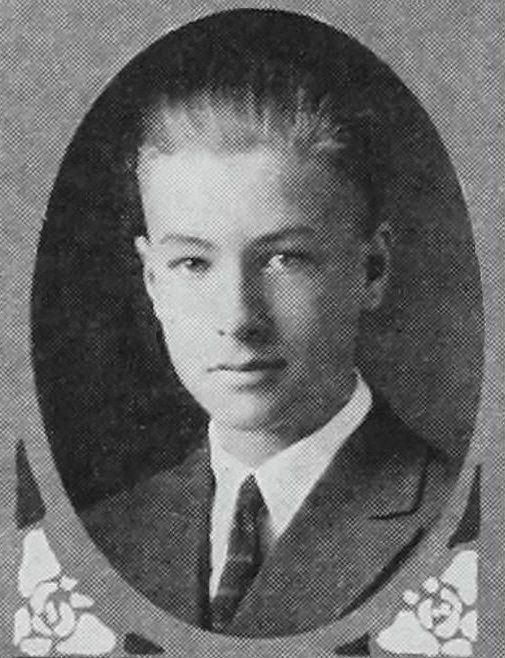
\includegraphics[scale=0.1]{./Figures/Howard Garns.jpeg}
		\caption{Howard Garns}
	\end{figure}
\end{frame}

\begin{frame}
	\frametitle{History(2)}
	\begin{itemize}
		\item \el Το \en SUDOKU \el έγινε ιδιαίτερα αγαπητό στην Ιαπωνία, με τις μηνιαίες πωλήσεις \en SUDOKU \el περιοδικών να ανέρχονται στα 600.000 αντίτυπα κάθε μήνα.
		\item Οι Ιάπωνες υιοθέτησαν το \en SUDOKU \el ως συνήθεια για δύο βασικούς λόγους: 
		\begin{itemize}
			\item η γλώσσα τους δεν ήταν κατάλληλη για την ανάπτυξη σταυρόλεξων, οπότε υστερούσαν σε αυτά και 
			\item συνηθίζουν να μετακινούνται με τρένα και λεωφορεία.
		\end{itemize}
	\end{itemize}
\end{frame}

\begin{frame}
	\frametitle{History(3)}
	\begin{figure}
		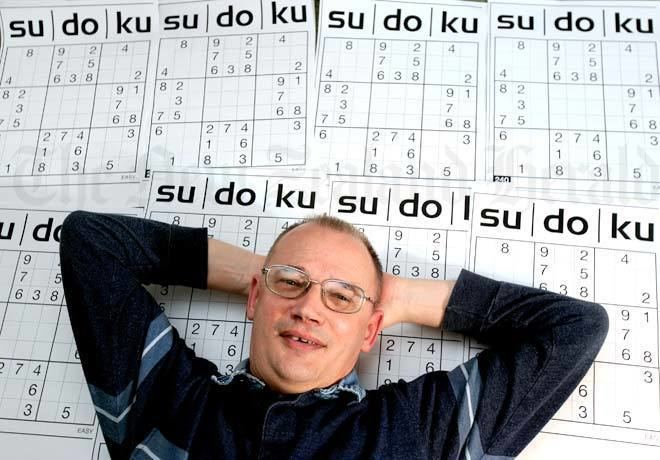
\includegraphics[scale=0.2]{./Figures/WayneGould.jpg}
		\caption{Wayne Gould}
	\end{figure}
	\begin{itemize}
		\item \el Ο \en Wayne Gould \el, Νεοζηλανδός δικαστής, έφερε πίσω στον Δυτικό κόσμο το \en SUDOKU. 
		\item \el To 1997 βρισκόταν στο Τόκιο και ανακάλυψε ενα \en SUDOKU. 
		\item \el Έφτιαξε το πρωτο πρόγραμμα που δημιουργούσε \en SUDOKU \el παζλ. 
	\end{itemize}
\end{frame}

	\begin{frame}
		\frametitle{Study}
		\el Στην παρούσα εργασία θα μελετήσουμε σε βάθος: \\

		\begin{itemize}
			\item \el Μαθηματικές μεθοδολογίες για την επίλυση \en sudoku.
				\begin{itemize}
					\item \el Μοντελοποίηση του προβλήματος της επίλυσης του παζλ ως πρόβλημα γραμμικού προγραμματισμού.
					\item Επαλήθευση με χρήση \en MATLAB .
					\item \el Παραλλαγές του κλασσικού \en sudoku.
				\end{itemize}
			\item \el Μαθηματικές τεχνικές για τη δημιουργία \en sudoku.
			\begin{itemize}
				\item \el Δημιουργία \en sudoku \el με \en bruteforce.
				\item \el Δημιουργία \en sudoku \el από παλαιότερο παζλ.
			\end{itemize}
		\end{itemize}
	\end{frame}

	\begin{frame}
	\frametitle{References(1)}
	\begin{itemize}
		\item \textit{J. F. Crook, A Pencil-and-Paper Algorithm for Solving Sudoku Puzzles, Notices of the AMS (April 2009)}
		\item \textit{Andrew C. Stuart, Sudoku Creation and Grading (February 2007 - updated January 2012)}
		\item \textit{Arnab Kumar Maji, Sunanda Jana, Sudipta Roy, Rajat Kumar Pal, An Exhaustive Study on different Sudoku Solving Techniques, International Journal of Computer Science Issues, Vol. 11, Issue 2, No 1, March 2014}
		\item \textit{Radek Pelánek, Human Problem Solving:Sudoku Case Study (January 2011)}
		\item \textit{Rohit Iyer, Amrish Jhaveri, Krutika Parab, A Review of Sudoku Solving using Patterns, International Journal of Scientific and Research Publications, Volume 3, Issue 5, May 2013}
		\item \textit{Rhyd Lewis, Metaheuristics can Solve Sudoku Puzzles}
	\end{itemize}
\end{frame}

	\begin{frame}
	\frametitle{References(2)}
	\begin{itemize}
		\item \textit{"The History of Sudoku",www.sudoku.com, https://sudoku.com/how-to-play/the-history-of-sudoku/}
	\end{itemize}
\end{frame}

\end{document}